\documentclass[]{article}
\usepackage{lmodern}
\usepackage{amssymb,amsmath}
\usepackage{ifxetex,ifluatex}
\usepackage{fixltx2e} % provides \textsubscript
\ifnum 0\ifxetex 1\fi\ifluatex 1\fi=0 % if pdftex
  \usepackage[T1]{fontenc}
  \usepackage[utf8]{inputenc}
\else % if luatex or xelatex
  \ifxetex
    \usepackage{mathspec}
  \else
    \usepackage{fontspec}
  \fi
  \defaultfontfeatures{Ligatures=TeX,Scale=MatchLowercase}
\fi
% use upquote if available, for straight quotes in verbatim environments
\IfFileExists{upquote.sty}{\usepackage{upquote}}{}
% use microtype if available
\IfFileExists{microtype.sty}{%
\usepackage{microtype}
\UseMicrotypeSet[protrusion]{basicmath} % disable protrusion for tt fonts
}{}
\usepackage[margin=1in]{geometry}
\usepackage{hyperref}
\hypersetup{unicode=true,
            pdftitle={videogamesScraper: Compilación de videojuegos Retro desde 1976 hasta 2018},
            pdfauthor={Ricardo Garcia Ruiz},
            pdfborder={0 0 0},
            breaklinks=true}
\urlstyle{same}  % don't use monospace font for urls
\usepackage{graphicx,grffile}
\makeatletter
\def\maxwidth{\ifdim\Gin@nat@width>\linewidth\linewidth\else\Gin@nat@width\fi}
\def\maxheight{\ifdim\Gin@nat@height>\textheight\textheight\else\Gin@nat@height\fi}
\makeatother
% Scale images if necessary, so that they will not overflow the page
% margins by default, and it is still possible to overwrite the defaults
% using explicit options in \includegraphics[width, height, ...]{}
\setkeys{Gin}{width=\maxwidth,height=\maxheight,keepaspectratio}
\IfFileExists{parskip.sty}{%
\usepackage{parskip}
}{% else
\setlength{\parindent}{0pt}
\setlength{\parskip}{6pt plus 2pt minus 1pt}
}
\setlength{\emergencystretch}{3em}  % prevent overfull lines
\providecommand{\tightlist}{%
  \setlength{\itemsep}{0pt}\setlength{\parskip}{0pt}}
\setcounter{secnumdepth}{5}
% Redefines (sub)paragraphs to behave more like sections
\ifx\paragraph\undefined\else
\let\oldparagraph\paragraph
\renewcommand{\paragraph}[1]{\oldparagraph{#1}\mbox{}}
\fi
\ifx\subparagraph\undefined\else
\let\oldsubparagraph\subparagraph
\renewcommand{\subparagraph}[1]{\oldsubparagraph{#1}\mbox{}}
\fi

%%% Use protect on footnotes to avoid problems with footnotes in titles
\let\rmarkdownfootnote\footnote%
\def\footnote{\protect\rmarkdownfootnote}

%%% Change title format to be more compact
\usepackage{titling}

% Create subtitle command for use in maketitle
\newcommand{\subtitle}[1]{
  \posttitle{
    \begin{center}\large#1\end{center}
    }
}

\setlength{\droptitle}{-2em}
  \title{videogamesScraper: Compilación de videojuegos Retro desde 1976 hasta
2018}
  \pretitle{\vspace{\droptitle}\centering\huge}
  \posttitle{\par}
  \author{Ricardo Garcia Ruiz}
  \preauthor{\centering\large\emph}
  \postauthor{\par}
  \predate{\centering\large\emph}
  \postdate{\par}
  \date{08 de Abril de 2018}


\begin{document}
\maketitle

{
\setcounter{tocdepth}{3}
\tableofcontents
}
\section{Características de la
práctica}\label{caracteristicas-de-la-practica}

\subsection{Presentación}\label{presentacion}

En esta práctica se elabora un caso práctico orientado a aprender a
identificar los datos relevantes por un proyecto analítico y usar las
herramientas de extracción de datos. Para hacer esta práctica tendréis
que trabajar en grupos de 3 o 2 personas, o si preferís, también podéis
hacerlo de manera individual. Tendréis que entregar un solo fichero con
el enlace Github (\url{https://github.com}) donde haya las soluciones
incluyendo los nombres de los componentes del equipo. Podéis utilizar la
Wiki de Github para describir vuestro equipo y los diferentes archivos
de vuestra entrega. Cada miembro del equipo tendrá que contribuir con su
usuario Github. Podéis mirar estos ejemplos como guía:

\begin{itemize}
\tightlist
\item
  Ejemplo: \url{https://github.com/rafoelhonrado/foodPriceScraper}
\item
  Ejemplo complejo: \url{https://github.com/tteguayco/Web-scraping}
\end{itemize}

\subsection{Objetivos}\label{objetivos}

Los objetivos concretos de esta práctica son:

\begin{itemize}
\tightlist
\item
  Aprender a aplicar los conocimientos adquiridos y su capacidad de
  resolución de problemas en entornos nuevos o poco conocidos dentro de
  contextos más amplios o multidisciplinarios.
\item
  Saber identificar los datos relevantes que su tratamiento aportan
  valor a una empresa y la identificación de nuevos proyectos
  analíticos.
\item
  Saber identificar los datos relevantes para llevar a cabo un proyecto
  analítico.
\item
  Capturar datos de diferentes fuentes de datos (tales como redes
  sociales, web de datos o repositorios) y mediante diferentes
  mecanismos (tales como queries, API y scraping).
\item
  Actuar con los principios éticos y legales relacionados con la
  manipulación de datos en función del ámbito de aplicación.
\item
  Desarrollar la capacidad de búsqueda, gestión y uso de información y
  recursos en el ámbito de la ciencia de datos.
\end{itemize}

\subsection{Descripción de la Práctica a
realizar}\label{descripcion-de-la-practica-a-realizar}

El objetivo de esta actividad será la creación de un dataset a partir de
los datos contenidos al web. Tenéis que indicar las siguientes
características del dataset general:

\begin{enumerate}
\def\labelenumi{\arabic{enumi}.}
\tightlist
\item
  Título del dataset. Poned un título que sea descriptivo.
\item
  Subtítulo del dataset. Agregad una descripción ágil de vuestro
  conjunto de datos por vuestro subtítulo.
\item
  Imagen. Agregad una imagen que identifique vuestro dataset visualmente
\item
  Contexto. ¿Cuál es la materia del conjunto de datos?
\item
  Contenido. ¿Qué campos incluye? ¿Cuál es el periodo de tiempo de los
  datos y cómo se ha recogido?
\item
  Agradecimientos. ¿Quién es propietario del conjunto de datos? Incluid
  citas de investigación o análisis anteriores.
\item
  Inspiración. ¿Por qué es interesante este conjunto de datos? ¿Qué
  preguntas le gustaría responder la comunidad?
\item
  Licencia. Seleccionad una de estas licencias y decid porqué la habéis
  seleccionado:
\end{enumerate}

\begin{itemize}
\tightlist
\item
  Released Under CC0: Public Domain License
\item
  Released Under CC BY-NC-SA 4.0 License
\item
  Released Under CC BY-SA 4.0 License
\item
  Database released under Open Database License, individual contents
  under Database Contents License
\item
  Other (specified above)
\item
  Unknown License
\end{itemize}

\begin{enumerate}
\def\labelenumi{\arabic{enumi}.}
\setcounter{enumi}{8}
\tightlist
\item
  Código: Hay que adjuntar el código con el que habéis generado el
  dataset, preferiblemente con R o Python, que os ha ayudado a generar
  el dataset
\item
  Dataset: Dataset en formato CSV
\end{enumerate}

\clearpage

\section{Realización de la práctica}\label{realizacion-de-la-practica}

\subsection{Título del dataset: Base de datos general de videojuegos
retro}\label{titulo-del-dataset-base-de-datos-general-de-videojuegos-retro}

Para construir nuestro dataset \textbf{Base de datos general de
videojuegos retro}, el conjunto de datos escogido para esta práctica ha
sido el de la web \url{http://www.retrocollect.com/}. Se pretende
compilar una base de datos de videojuegos retro, y despues de un
exhaustivo análisis de las diversas compilaciones de videojuegos retro
existentes en Internet, se ha escogido la que ofrece RetroCollect, que
corresponde con videojuegos de los denominados \textbf{`retro'}, y que
ha resultado ser amplia y diversificada.

Logotipo de RetroCollect extraído de \url{http://www.retrocollect.com/}

\begin{figure}[h!]
\centering

\includegraphics{RetroCollect-Logo.png}
\end{figure}

El periodo de datos que abarca la base de datos está entre 1976 y 2018,
existiendo algunos videojuegos que no están correctamente datados en la
própia página web.

Las principales variables de este conjunto corresponden con la
\textbf{fecha}, el \textbf{nombre} del videojuego y la
\textbf{plataforma} de juegos.

\subsection{Imagen identificativa}\label{imagen-identificativa}

Protagonistas del videojuego iconico por excelencia: Mario Bros.

Cortesía de Alexas,
\url{https://pixabay.com/es/mario-luigi-yoschi-cifras-gracioso-1557240/}

\begin{figure}[h!]
  \centering
  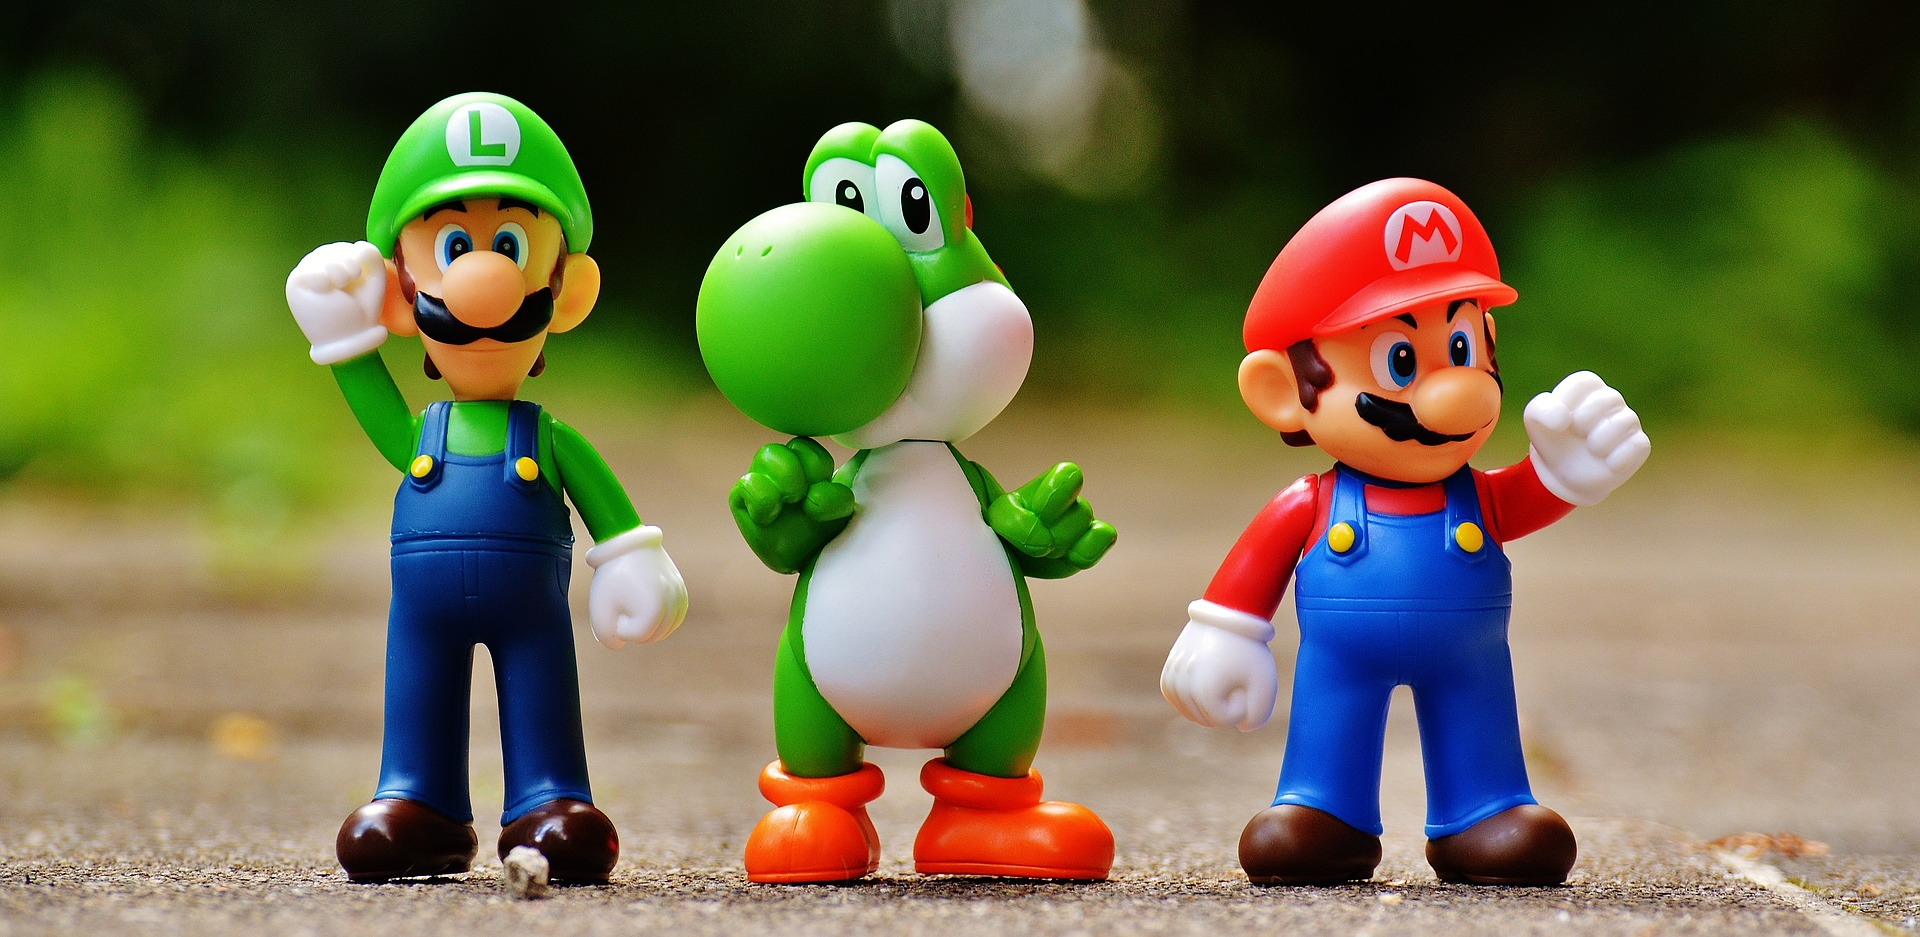
\includegraphics[width=.8\textwidth]{mario-1557240_1920.jpg}
\end{figure}

\subsection{Contexto}\label{contexto}

El conjunto de datos se corresponde con videojuegos de tipo
\emph{`retro'} que se hayan poblicado en un periodó que abarca 1976 al
2018. Aunque existen videojuegos que abarcan desde los años 50, estos
son considerados como \emph{arcanos}, y en algunos casos no son mas que
prototipos de los juegos que verdaderamente empezaron a comercializarse
en la década de los 70 del siglo pasado.

Entre ellos pueden encontrarse todo tipo de géneros:

\begin{itemize}
\tightlist
\item
  Action
\item
  Adventure
\item
  Compilation
\item
  DLC
\item
  Add-on
\item
  Educational
\item
  Puzzle
\item
  Racing
\item
  Driving
\item
  Role-Playing (RPG)
\item
  Simulation
\item
  Special Edition
\item
  Sports
\item
  Strategy/Tactics
\end{itemize}

\subsection{Contenido}\label{contenido}

Para cada videojuego, el cual se corresponde con un registro en el
conjunto de datos, se recogen las siguientes características:

\begin{enumerate}
\def\labelenumi{\arabic{enumi}.}
\tightlist
\item
  \textbf{Original System}: .
\item
  \textbf{Title}: Titulo original del videojuego (en ingles).
\item
  \textbf{Year}: año de publicación del videojuego.
\item
  \textbf{Publisher}: compañía que lo lanzó al mercado comercial en el
  año citado.
\item
  \textbf{Developer}: compañía desarrolladora del videojuego. Puede
  coincidir en algunos casos con el \emph{`Publisher'} pero es
  importante, ya que en los 70, 80 y 90 del siglo pasado había muchas
  compañías que desarrollaban los juegos por encargo.
\item
  \textbf{Países de lanzamiento}: Se agrupan en tres categorías (Europe,
  US y Japan). Cada registro puede estar vacío o con una \textbf{`x'}.
  La \textbf{`x'} indica que en ese país o región no fue comercializado:

  \begin{enumerate}
  \def\labelenumii{\arabic{enumii}.}
  \tightlist
  \item
    \textbf{Europe}: cualquier país de Europa.\\
  \item
    \textbf{US}: en Estados Unidos.\\
  \item
    \textbf{Japan}: en Japón.
  \end{enumerate}
\end{enumerate}

\emph{RetroCollect} solo almacena datos de juegos que se consideran
\textbf{`retro'}, de forma que aunque algunos juegos puedan ser
sobradamente conocidos, deben alcanzar la categoría de \textbf{`retro'}
para poder estar incluídos en esta web.

Existen otras web que compilan datos sobre videojuegos, pero la
extracción de datos únicamente de videojuegos \emph{retro} requería de
un tratamiento posterior que no es el objetivo de esta práctica, sino el
adquirir los datos directamente de la web.

\clearpage

\subsubsection{Ficheros del código
fuente}\label{ficheros-del-codigo-fuente}

\begin{enumerate}
\def\labelenumi{\arabic{enumi}.}
\tightlist
\item
  \textbf{src/videogamesScraper}: Es el código de entrada al scraping y
  contiene el código principal utilizado para gestionar el trabajo de
  compilación de toda la base de datos retro de videojuegos de la web
  \textbf{RetroCollect}.
\item
  \textbf{src/getPlatformDB}: Contiene el código fuente de la función
  \textbf{getPlatformDB()}. Esta función accede a la web de RetroCollet
  y obtiene un data frame con los códigos numérícos y sus equivalencias
  en texto de los nombres de las Plataformas disponibles en
  RetroCollect. Con esta función se puede realizar un filtro por tipo de
  plataforma, o bien toda la base de datos de videojuegos (por defecto).
\item
  \textbf{src/searchPaginationDB}: Contiene el código fuente de la
  función \textbf{searchPaginationDB()}. La función realiza una búsqueda
  en la web localizando la página web última en la que se deben buscar
  los datos de scraping, devolviendo un valor numérico con la última
  página que se debe acceder. Los paramétros son los siguientes:

  \begin{itemize}
  \tightlist
  \item
    \textbf{url\_base}: La dirección web generalde acceso a RetroCollect
  \item
    \textbf{listview}: Sistema de visualización, por defecto
    \emph{`list'}
  \item
    \textbf{modeview}: Por defecto se buscan \emph{`games'}
  \item
    \textbf{plataforma}: La plataforma de filtro, por defecto = 0, todas
    sin excepcion
  \item
    \textbf{sort}: Esquema de ordenación, puede tomar 4 parámetros:

    \begin{itemize}
    \tightlist
    \item
      \emph{`title'}, es el defectivo y es igual a \textbf{NA}
    \item
      \emph{`system'}, organiza por S.O. y es igual a
      \emph{``platform''}
    \item
      \emph{`publisher'}, organiza por cia. de publicación y es igual a
      \emph{``publisher''}
    \item
      \emph{`year'}, organiza por año de publicación y es igual a
      \emph{``year''}
    \end{itemize}
  \item
    \textbf{filas}: Indica el numero de filas de visualización por
    página, defecto = 20
  \item
    \textbf{verbose}: Indica si se desea o no información de progreso,
    defecto = \emph{TRUE}
  \end{itemize}
\item
  \textbf{src/accessVideoGameDatabase}: Contiene el código fuente de la
  función \textbf{accessVideoGameDatabase()}. La función realiza un web
  scrapin en RetroCollect, posibilitando un acceso dinamico a la misma y
  configurando algunos parametros de control en la llamada a la pagina
  web de RetroCollect indicando algunas variables de carga y control de
  visualización. Los paramétros son los siguientes:

  \begin{itemize}
  \tightlist
  \item
    \textbf{url\_base}: La dirección web generalde acceso a RetroCollect
  \item
    \textbf{listview}: Sistema de visualización, por defecto
    \emph{`list'}
  \item
    \textbf{modeview}: Por defecto se buscan \emph{`games'}
  \item
    \textbf{plataforma}: La plataforma de filtro, por defecto = 0, todas
    sin excepcion
  \item
    \textbf{sort}: Esquema de ordenación, puede tomar 4 parámetros:

    \begin{itemize}
    \tightlist
    \item
      \emph{`title'}, es el defectivo y es igual a \textbf{NA}
    \item
      \emph{`system'}, organiza por S.O. y es igual a
      \emph{``platform''}
    \item
      \emph{`publisher'}, organiza por cia. de publicación y es igual a
      \emph{``publisher''}
    \item
      \emph{`year'}, organiza por año de publicación y es igual a
      \emph{``year''}
    \end{itemize}
  \item
    \textbf{filas}: Indica el numero de filas de visualización por
    página, defecto = 20
  \item
    \textbf{verbose}: Indica si se desea o no información de progreso,
    defecto = \emph{TRUE}
  \end{itemize}
\end{enumerate}

\subsection{Agradecimientos}\label{agradecimientos}

Los datos han sido compilados desde la base de datos online
\href{http://www.retrocollect.com/}{RetroCollect}. Se ha utilizado el
lenguaje `\textbf{R}' y de técnicas de \emph{Web Scraping} para extraer
la información alojada en las múltiples páginas de gestión de esta base
de datos online.

En la presentación de este trabajo se han utilizado referencias a los
siguientes trabajos:

\begin{enumerate}
\def\labelenumi{\arabic{enumi}.}
\tightlist
\item
  Simon Munzert, Christian Rubba, Peter Meißner, Dominic Nyhuis. (2015).
  \emph{Automated Data Collection with R: A Practical Guide to Web
  Scraping and Text Mining.} John Wiley \& Sons
\item
  Garcia Ruiz, Ricardo. (2014). \emph{Estudio y caracterización de
  marcas de videojuegos mediante análisis de la producción de patentes y
  el desarrollo técnico de software para plataformas de videojuegos.}
  Universitat Internacional de Catalunya, DOI: 10.13140/2.1.5162.0166.
\end{enumerate}

\subsection{Inspiración}\label{inspiracion}

El conjunto de datos puede resultar muy útil para trabajos relacionados
con la minería de datos relativa al comportamiento de los videojuegos
(García Ruiz 2014).

Tambien sirve para verificar el comportamiento analítico sobre los
desarrolladores y publicadores de videojuegos a lo largo del tiempo.

De igual manera, también puede utilizar verificar el comportamiento de
aceptación de los diversos videojuegos a lo largo del tiempo en las
distintas zonas geográficas, y su impacto relativo o absoluto.

\subsection{Licencia}\label{licencia}

La licencia escogida para la publicación de este conjunto de datos ha
sido \textbf{CC BY-NC-SA 4.0 ES}. Los motivos que han llevado a la
elección de esta licencia tienen que ver con la idoneidad de las
cláusulas que esta presenta en relación con el trabajo realizado:

Se permite con nuestro trabajo y la base de datos extraída de la web:

\begin{itemize}
\tightlist
\item
  \emph{Compartir} --- copiar y redistribuir el material en cualquier
  medio o formato
\item
  \emph{Adaptar} --- remezclar, transformar y crear a partir del
  material
\end{itemize}

Por otro lado, la licencia activa las siguientes restricciones:

\begin{itemize}
\tightlist
\item
  \textbf{Reconocimiento}: Debe reconocer adecuadamente la autoría,
  proporcionar un enlace a la licencia e indicar si se han realizado
  cambios. Puede hacerlo de cualquier manera razonable, pero no de una
  manera que sugiera que tiene el apoyo del licenciador o lo recibe por
  el uso que hace.
\item
  \textbf{NoComercial}: No puede utilizar el material para una finalidad
  comercial.
\item
  \textbf{CompartirIgual}: Si remezcla, transforma o crea a partir del
  material, deberá difundir sus contribuciones bajo la misma licencia
  que el original.
\item
  \textbf{No hay restricciones adicionales}: No puede aplicar términos
  legales o medidas tecnológicas que legalmente restrinjan realizar
  aquello que la licencia permite.
\end{itemize}

\subsection{Código fuente y dataset}\label{codigo-fuente-y-dataset}

Tanto el código fuente escrito para la extracción de datos como el
dataset generado pueden ser accedidos a través de
\href{https://github.com/rgarciarui/videogamesScrapper}{este enlace}.

Para el desarrollo de la práctica se han tomado en consideración las
técnicas de Web Scraping de (Munzert et al. 2014).

\subsection*{Recursos}\label{recursos}
\addcontentsline{toc}{subsection}{Recursos}

\hypertarget{refs}{}
\hypertarget{ref-ruiz2014estudio}{}
García Ruiz, Ricardo. 2014. ``Estudio Y Caracterización de Marcas de
Videojuegos Mediante análisis de La Produccion de Patentes Y El
Desarrollo Técnico de Software Para Plataformas de Videojuegos.''
PhD thesis, Universitat Internacional de Catalunya.

\hypertarget{ref-munzert2014automated}{}
Munzert, Simon, Christian Rubba, Peter Meißner, and Dominic Nyhuis.
2014. \emph{Automated Data Collection with R: A Practical Guide to Web
Scraping and Text Mining}. John Wiley \& Sons.


\end{document}
